\chapter{Preliminaries}

%%%%%%%%%%%%%%%%%%%%%%
\section{Introduction}
In mathematics, one uses groups to study symmetry.  In particular, a reflection group can be used to study the reflection and rotational symmetry of an object.  A Coxeter group can be thought of as a generalized reflection group, where the group is generated by a set of elements of order two (i.e., reflections) and there are rules for how the generators interact with each other.  Every element of a Coxeter group can be written as an expression in the generators, and if the number of generators in an expression (including multiplicity) is minimal, we say that the expression is reduced. Kazhdan--Lusztig polynomials arise in the context of Hecke algebras associated to Coxeter groups. The computation of these polynomials is very difficult for examples of even moderate rank. Motivated by the desire to understand these Kazhdan--Lusztig theory of the Hecke algebra of the underlying Coxeter group, Green~\cite{Green2006a} classified the so-called star reducible Coxeter groups which have the property that all fully commutative elements (in the sense of Stembridge) can be sequentially reduced via star operations to a product of commuting generators. It turns out that in some Coxeter groups there are elements, called T-avoiding elements, which cannot be systematically dismantled in the way described above. More specifically an element $w$ is called \emph{T-avoiding} if $w$ does not have a reduced expression beginning or ending with a pair of non-commuting generators. Clearly, a product of commuting generators is trivially T-avoiding. However, sometimes there are more interesting T-avoiding elements, which we will refer to as type 2 T-avoiding elements. Our motivation for studying the T-avoiding elements stems from Kazhdan--Lusztig polynomials, denoted by $P_{x,w}$. Specifically a bound on the degree of $P_{x,w}$ is known but in general it is not known when this bound is achieved. Of particular interest is the leading coefficient $\mu(x,w)$ which appears when the maximum degree of $P_{x,w}$. These coefficients are determined through a recurrence relations, however no closed form is known for calculating these in an efficient matter. Coxeter groups that have type 2 T-avoiding elements leads to the calculation becoming more difficult as the descent sets of these elements have undesirable properties. Specifically, when $x$ is a type 2 T-avoiding element and $w$ is fully commutative the properties make the calculations even more difficult. In addition to the above the computations involving the elements of the generalized Temperly--Lieb algebra for $W$ that are indexed by T-avoiding elements is ``well-behaved." In fact, knowing which elements correspond to T-avoiding elements often provides us with the base case for inductive arguments involving star operations.

In his PhD thesis~\cite{Gern2013a}, Gern classified the T-avoiding elements in Coxeter groups of type $D_n$. Unlike in types $A_n$ and $B_n$, it turns out that the classification in type $D_n$ includes non-trivial T-avoiding elements. The T-avoiding elements are rich in combinatorics and are interesting in their own right. The focus of this thesis is identifying T-avoiding elements in certain Coxeter groups.

This thesis is organized as follows. After necessary background information is presented in Section~\ref{sec:coxeter}, we introduce the class of fully commutative elements in Section~\ref{sec:FC}. Next in Section~\ref{sec:Heaps} we discuss a visual representation for elements of Coxeter groups, called heaps. In Section~\ref{sec:star}, we introduce the concept of a star reduction and star reducible Coxeter groups and in Section~\ref{sec:Tavoid} we formally introduce the notion of a T-avoiding element. In Section~\ref{sec:noncancel} we define the notion of a non-cancellable element in Coxeter groups, as well as remark upon a specific family of non-cancellable elements in $W(\C_n)$ when $n$ is odd. We then state classifications and conjectures regarding T-avoiding elements in several Coxeter groups in Chapter~\ref{chap:TandTavoid}. All of these results, barring Section~\ref{sec:tavoidI}, are previously known. Chapters~\ref{chap:BnandCn} and~\ref{chap:Cn} contain the main results of this thesis, namely the classification of T-avoiding elements in Coxeter groups of types $B_n$ and $\C_n$, which are new results. In Section~\ref{sec:Btools}, we introduce the necessary lemmas and definitions for the classification in Section~\ref{sec:TAB}, in which we show there are no non-trivial T-avoiding elements in Coxeter groups of type $B_n$. In Section~\ref{sec:TAC}, we classify the type II T-avoiding elements in Coxeter groups of type $\C_n$. We conclude with some open questions in Section~\ref{sec:open}.


%%%%%%%%%%%%%%%%%%%%%%%%%

\section{Coxeter Systems}\label{sec:coxeter}

A \emph{Coxeter system} is a pair $(W,S)$ consisting of a finite set $S$ of generating involutions and a group $W$, called a \emph{Coxeter group}, with presentation 
\[ 
W = \langle S \mid (st)^{m(s, t)} = e  \rangle,
\]
where $e$ is the identity, $m(s,t) = 1$ if and only if $s = t$, and $m(s,t) = m(t,s) \geq 2$ for $s \neq t$. If there is no relation between $s,t \in S$, then we define $m(s,t)=\infty$. However, in this thesis we assume that all $m(s,t)$ are finite. It turns out that the elements of $S$ are distinct as group elements and that $m(s,t)$ is the \emph\emph{order} of $st$~\cite{Humphreys1990}. We call $m(s,t)$ the \emph{bond strength} of $s$ and $t$.\\

Since $s$ and $t$ are elements of order 2, the relation $(st)^{m(s,t)}=e$ can be rewritten as
\begin{equation}\label{braid} 
	\underbrace{sts \cdots}_{m(s,t)}=\underbrace{tst\cdots}_{m(s,t)}
\end{equation}
with $m(s,t) \geq 2$ factors. If $m(s,t)=2$, then $st=ts$ is called a \emph{commutation relation}. Otherwise, if $m(s,t) \geq 3$, then the relation in \eqref{braid} is called a \emph{braid relation}. The replacement \[\underbrace{sts\cdots}_{m(s,t)} \mapsto  \underbrace{tst\cdots}_{m(s,t)}\] will be referred to as a \emph{commutation} if $m(s,t)=2$ and a \emph{braid move} if $m(s,t) \geq 3$.\\

We can represent a Coxeter system $(W,S)$ with a \emph{Coxeter graph} $\Gamma$ having
\begin{enumerate}[leftmargin=2cm]
\item vertex set $S$ and
\item edges $\{s, t\}$ for each $m(s,t) \geq 3$.	
\end{enumerate}

Each edge $\{s,t\}$ is labeled with its corresponding bond strength. Since $m(s,t)=3$ occurs frequently, it is customary to omit this label. Note that $s$ and $t$ are not connected by an edge in the graph if and only if $m(s,t)=2$. There is a one-to-one correspondence between Coxeter systems and Coxeter graphs. That is, given a Coxeter graph $\Gamma$, we can uniquely reconstruct the corresponding Coxeter system. If $(W,S)$ is a Coxeter system with corresponding Coxeter graph $\Gamma$, we may denote the Coxeter group as $W(\Gamma)$ and the generating set as $S(\Gamma)$ for clarity. Also, the Coxeter system $(W,S)$ is said to be \emph{irreducible} if and only if $\Gamma$ is connected. If the graph $\Gamma$ is disconnected, the connected components correspond to factors in a direct product of the corresponding Coxeter groups~\cite{Humphreys1990}. The Coxeter graphs given in Figure~\ref{fig:labeledgraphs} correspond to the Coxeter systems that will be primarily addressed in this thesis. 

\begin{figure}[h]
\begin{tabular}{m{7cm} m{7cm}}
\begin{subfigure}{0.5\textwidth} \centering
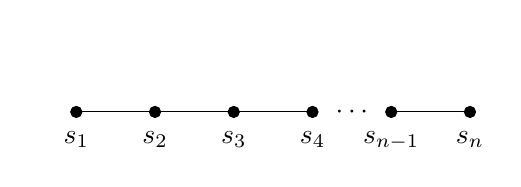
\begin{tikzpicture}[scale=1.0]%A_{n}
\draw[fill=black] \foreach \x in {1,2,...,6} {(\x,10) circle (2pt)};
\fill[fill=white] (2,11) circle (2pt);
\draw {(.5,10) node{}
(1.5,10) node[label=above:\textcolor{white}{$4$}]{}
(4.5,10) node{$\cdots$}
(1,10) node[label=below:$s_1$]{}
(2,10) node[label=below:$s_2$]{}
(3,10) node[label=below:$s_3$]{}
(4,10) node[label=below:$s_4$]{}
(5,10) node[label=below:$s_{n-1}$]{}
(6,10) node[label=below:$s_{n}$]{}
[-] (1,10) -- (4,10)
[-] (5,10) -- (6,10)
(1,10) node{}}; 
\end{tikzpicture}
\caption{$A_{n}$} \label{fig:labeledA}
\end{subfigure} &

\begin{subfigure}{0.5\textwidth} \centering
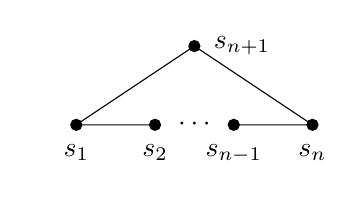
\begin{tikzpicture}[scale=1.0]%\widetilde{A}_{n}
\draw [fill=black] \foreach \x in {1,...,4} {(\x,7.5) circle (2pt)};
\draw [fill=black] (2.5, 8.5) circle (2pt);
\draw {(.5,8.5) node{}
(2.5,7.5) node{$\cdots$}
(1,7.5) node[label=below:$s_1$]{}
(2,7.5) node[label=below:$s_2$]{}
(3,7.5) node[label=below:$s_{n-1}$]{}
(4,7.5) node[label=below:$s_{n}$]{}
(2.5,8.5) node[label=right:$s_{n+1}$]{}
[-] (2.5,8.5) -- (1, 7.5)
[-] (2.5,8.5) -- (4, 7.5)
[-] (1,7.5) -- (2,7.5)
[-] (3,7.5) -- (4,7.5)
(2,8.5) node{}}; 
\end{tikzpicture}
\caption{$\widetilde{A}_{n}$} \label{fig:labeledaffAn}
\end{subfigure} \\

    & \\ 

\begin{subfigure}{0.5\textwidth} \centering
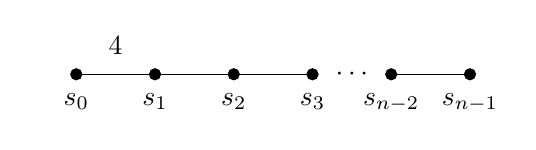
\begin{tikzpicture}[scale=1.0]%B_{n}
\draw [fill=black] \foreach \x in {1,2,...,6} {(\x,8.5) circle (2pt)};
%\draw [fill=white] (1,10) circle(2pt);
\draw {(.5,8.5) node{}
(1.5,8.5) node[label=above:$4$]{}
(6,8.5) node[label=above:\textcolor{white}{$4$}]{}
(4.5,8.5) node{$\cdots$}
(1,8.5) node[label=below:$s_0$]{}
(2,8.5) node[label=below:$s_1$]{}
(3,8.5) node[label=below:$s_2$]{}
(4,8.5) node[label=below:$s_3$]{}
(5,8.5) node[label=below:$s_{n-2}$]{}
(6,8.5) node[label=below:$s_{n-1}$]{}
[-] (1,8.5) -- (4,8.5)
[-] (5,8.5) -- (6,8.5)
(2,8.5) node{}}; 
\end{tikzpicture}
\caption{$B_{n}$} \label{fig:labeledB}
\end{subfigure} &

\begin{subfigure}{0.5\textwidth} \centering
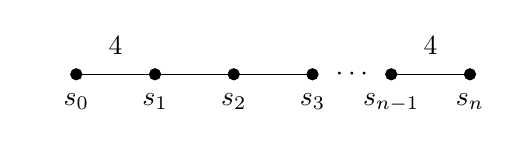
\begin{tikzpicture}[scale=1.0]
\draw[fill=black] \foreach \x in {1,2,...,6} {(\x,5) circle (2pt)};%\widetild{C}_{n}
%\fill[white] (1,6) circle (2pt);
\draw {(.5,5) node{}
(4.5,5) node{$\cdots$}
(5.5,5) node[label=above:$4$]{}
(1.5,5) node[label=above:$4$]{}
(1,5) node[label=below:$s_0$]{}
(2,5) node[label=below:$s_1$]{}
(3,5) node[label=below:$s_2$]{}
(4,5) node[label=below:$s_3$]{}
(5,5) node[label=below:$s_{n-1}$]{}
(6,5) node[label=below:$s_{n}$]{}
[-] (1,5) -- (4,5)
[-] (5,5) -- (6,5)
(2,5) node{}};
\end{tikzpicture}
\caption{$\widetilde{C}_{n}$} \label{fig:labeledaffC}
\end{subfigure}  \\

& \\

\begin{subfigure}{0.5\textwidth} \centering
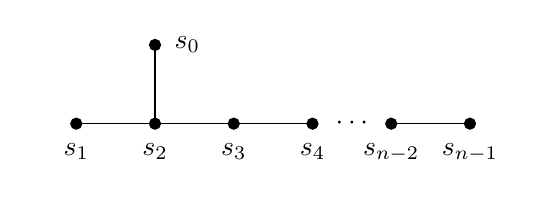
\begin{tikzpicture}[scale=1.0]
\draw[fill=black] \foreach \x in {1,2,...,6} {(\x,6.5) circle (2pt)};%D_{n}
\draw[fill=black] (2,7.5) circle (2pt);
\draw {(.5,6.5) node{}
(4.5,6.5) node{$\cdots$}
(1,6.5) node[label=below:$s_1$]{}
(2,6.5) node[label=below:$s_2$]{}
(3,6.5) node[label=below:$s_3$]{}
(4,6.5) node[label=below:$s_4$]{}
(5,6.5) node[label=below:$s_{n-2}$]{}
(6,6.5) node[label=below:$s_{n-1}$]{}
(2,7.5) node[label=right:$s_0$]{}
[-] (1,6.5) -- (4,6.5)
[-] (5,6.5) -- (6,6.5)
[-] (2,6.5) -- (2,7.5)
(2,6.5) node{}};
\end{tikzpicture}
\caption{$D_{n}$} \label{fig:labeledD}
\end{subfigure}&

\begin{subfigure}{0.5\textwidth} \centering
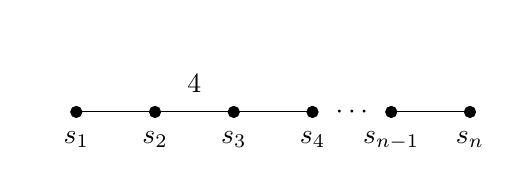
\begin{tikzpicture}[scale=1.0]%F_{n}
\draw[fill=black] \foreach \x in {1,2,...,6} {(\x,3) circle (2pt)};
\fill[white] (1,4) circle (2pt);
\draw {(.5,3) node{}
(2.5,3) node[label=above:$4$]{}
(4.5,3) node{$\cdots$}
(1,3) node[label=below:$s_1$]{}
(2,3) node[label=below:$s_2$]{}
(3,3) node[label=below:$s_3$]{}
(4,3) node[label=below:$s_4$]{}
(5,3) node[label=below:$s_{n-1}$]{}
(6,3) node[label=below:$s_{n}$]{}
[-] (1,3) -- (4,3)
[-] (5,3) -- (6,3)
(3,3) node{}};
\end{tikzpicture}
\caption{$F_{n}$} \label{fig:labeledFn}
\end{subfigure}  \\
\end{tabular}

\begin{subfigure}{1.0\textwidth} \centering
\begin{tikzpicture}[scale=1.0]
\draw[fill=black] \foreach \x in {1,2} {(\x,0) circle (2pt)};
\fill[fill=white] (2,1) circle (2pt);
\draw {(.25,0) node{}
(1.5,0) node[label=above:$m$]{}
(1,0) node[label=below:$s_1$]{}
(2,0) node[label=below:$s_2$]{}
[-] (1,0) -- (2,0)
(2,0) node{}};
\end{tikzpicture}
\caption{$I_{2}(m)$} \label{fig:labeledI}
\end{subfigure}

\caption{Examples of a few Coxeter graphs.}\label{fig:labeledgraphs}
\end{figure}


\begin{example}
~
\begin{itemize}
\item[(a)~] The Coxeter system of type $A_n$ is given by the graph in Figure~\ref{fig:labeledA}. We can construct the corresponding Coxeter group $W(A_n)$ with generating set $S(A_n)=\{s_1, s_2, \ldots ,s_n\}$ and defining relations
\begin{enumerate}[leftmargin=2cm]
	\item $s_i^2=e$ for all $i$;
	\item $s_is_j=s_js_i$ when $|i-j|>1$;
	\item $s_is_js_i=s_js_is_j$ when $|i-j|=1.$
\end{enumerate}
The Coxeter group $W(A_n)$ is isomorphic to the symmetric group $\Sym_{n+1}$ under the correspondence $s_i \mapsto (i, i+1)$, where $(i, i+1)$ is the adjacent transposition that swaps $i$ and $i+1$.
\item[(b)~]\label{ex:B} The Coxeter system of type $B_n$ is given by the graph in Figure~\ref{fig:labeledB}. We can construct the corresponding Coxeter group $W(B_n)$ with generating set $S(B_n)=\{s_0,s_1, \ldots ,s_{n-1}\}$ and defining relations
\begin{enumerate}[leftmargin=2cm]
	\item $s_i^2=e$ for all $i$;
	\item $s_is_j=s_js_i$  when $|i-j|>1$;
	\item $s_is_js_i=s_js_is_j$ when $|i-j|=1$ for $i,j \in \{1,2,\ldots, n-1\}$;
	\item $s_0s_1s_0s_1=s_1s_0s_1s_0$.
\end{enumerate}
The Coxeter group $W(B_n)$ is isomorphic to the group, $\Sym_n^B$, of signed permutations on the set $\{1,2, \ldots,n\}$. We discuss $\Sym_n^B$ in more detail in Section~\ref{sec:Btools}.
\item[(c)~] The Coxeter system of type $\widetilde C_n$ is given by the graph in Figure~\ref{fig:labeledaffC}. We can construct the corresponding Coxeter group $W(\widetilde C_n)$ with generating set $S(\widetilde{C}_n)=~\{s_0, s_1, \ldots ,s_n\}$ and defining relations 
\begin{enumerate}[leftmargin=2cm]
	\item $s_i^2=e$ for all $i$;
	\item $s_is_j=s_js_i$ when $|i-j|>1$ for $i \in \{0,2, \ldots, n\}$;
	\item $s_is_js_i=s_js_is_j$ 	when $|i-j|=1$ for $i \in \{1,2, \ldots, n-1\}$;
	\item $s_0s_1s_0s_1=s_1s_0s_1s_0$;
	\item $s_ns_{n-1}s_ns_{n-1}=s_{n-1}s_ns_{n-1}s_n.$
\end{enumerate}
Note that $W(\widetilde{C}_n)$ has $n+1$ generators. It turns out that $W(\C_n)$ is an infinite group.
\end{itemize}
\end{example}



The Coxeter graphs given in Figure~\ref{fig:fincoxgraphs} correspond to the collection of irreducible finite-type Coxeter systems, whose corresponding Coxeter groups are finite, while the Coxeter graphs given in Figure~\ref{fig:infincoxgraphs} are the so-called irreducible \emph{affine Coxeter systems}, whose corresponding Coxeter groups are infinite~\cite{Humphreys1990}. From now on we will refer to a finite Coxeter system to be a system where $W(\Gamma)$ is finite. Note that $W(B_n)$ is one of the irreducible finite Coxeter groups, so it is finite, while $W(\C_n)$ is one of the affine groups making it infinite. The irreducible affine Coxeter systems are unique in that if a vertex is removed along with the corresponding edges from the Coxeter graph, the newly created graph will result in a Coxeter system with a finite Coxeter group. 

\begin{figure}[h!]
\begin{tabular}{m{7cm} m{7cm}}
\begin{subfigure}{0.5\textwidth} \centering
\begin{tikzpicture}[scale=1.0]%A_{n}
\draw[fill=black] \foreach \x in {1,2,...,6} {(\x,10) circle (2pt)};
\draw {(.5,10) node{}
(1.5,10) node[label=above:\textcolor{white}{$4$}]{}
(4.5,10) node{$\cdots$}
%(1,10) node[label=below:$s_1$]{}
%(2,10) node[label=below:$s_2$]{}
%(3,10) node[label=below:$s_3$]{}
%(4,10) node[label=below:$s_4$]{}
%(5,10) node[label=below:$s_{n-1}$]{}
%(6,10) node[label=below:$s_{n}$]{}
[-] (1,10) -- (4,10)
[-] (5,10) -- (6,10)
(1,10) node{}}; 
\end{tikzpicture}
\caption{$A_{n}$} \label{fig:A}
\end{subfigure} &

\begin{subfigure}{0.5\textwidth} \centering
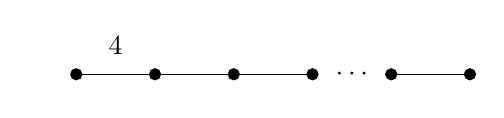
\begin{tikzpicture}[scale=1.0]%B_{n}
\draw [fill=black] \foreach \x in {1,2,...,6} {(\x,8.5) circle (2pt)};
\draw {(.5,8.5) node{}
(1.5,8.5) node[label=above:$4$]{}
(4.5,8.5) node{$\cdots$}
%(1,8.5) node[label=below:$s_0$]{}
%(2,8.5) node[label=below:$s_1$]{}
%(3,8.5) node[label=below:$s_2$]{}
%(4,8.5) node[label=below:$s_3$]{}
%(5,8.5) node[label=below:$s_{n-2}$]{}
%(6,8.5) node[label=below:$s_{n-1}$]{}
[-] (1,8.5) -- (4,8.5)
[-] (5,8.5) -- (6,8.5)
(2,8.5) node{}}; 
\end{tikzpicture}
\caption{$B_{n}$} \label{fig:B}
\end{subfigure} \\

    & \\ 

\begin{subfigure}{0.5\textwidth} \centering
\begin{tikzpicture}[scale=1.0]
\draw[fill=black] \foreach \x in {1,2} {(\x,0) circle (2pt)};
\fill[fill=white] (2,1) circle (2pt);
\draw {(.25,0) node{}
(1.5,0) node[label=above:$m$]{}
%(1,0) node[label=below:$s_1$]{}
%(2,0) node[label=below:$s_2$]{}
[-] (1,0) -- (2,0)
(2,0) node{}};
\end{tikzpicture}
\caption{$I_{2}(m)$} \label{fig:I}
\end{subfigure} &

\begin{subfigure}{0.5\textwidth} \centering
\begin{tikzpicture}[scale=1.0]
\draw[fill=black] \foreach \x in {1,2,...,6} {(\x,6.5) circle (2pt)};%D_{n}
\draw[fill=black] (2,7.5) circle (2pt);
\draw {(.5,6.5) node{}
(4.5,6.5) node{$\cdots$}
%(1,6.5) node[label=below:$s_1$]{}
%(2,6.5) node[label=below:$s_2$]{}
%(3,6.5) node[label=below:$s_3$]{}
%(4,6.5) node[label=below:$s_4$]{}
%(5,6.5) node[label=below:$s_{n-2}$]{}
%(6,6.5) node[label=below:$s_{n-1}$]{}
%(2,7.5) node[label=right:$s_0$]{}
[-] (1,6.5) -- (4,6.5)
[-] (5,6.5) -- (6,6.5)
[-] (2,6.5) -- (2,7.5)
(2,6.5) node{}};
\end{tikzpicture}
\caption{$D_{n}$} \label{fig:D}
\end{subfigure} \\

    & \\ 
    
\begin{subfigure}{0.5\textwidth} \centering
\begin{tikzpicture}[scale=1.0]%E_{6}
\draw[fill=black] \foreach \x in {1,2,...,5} {(\x,4.5) circle (2pt)};
\draw[fill=black] (3,5.5) circle (2pt);
\draw {
[-] (1,4.5) -- (5,4.5)
[-] (3,4.5) -- (3,5.5)
(3,4.5) node{}};
\end{tikzpicture}
\caption{$E_{6}$} \label{fig:E6}
\end{subfigure} &



\begin{subfigure}{0.5\textwidth} \centering
\begin{tikzpicture}[scale=1.0]%E_{7}
\draw[fill=black] \foreach \x in {1,2,...,6} {(\x,4.5) circle (2pt)};
\draw[fill=black] (3, 5.5) circle (2pt);
\draw {
[-] (1,4.5) -- (5,4.5)
[-] (5,4.5) -- (6,4.5)
[-] (3,4.5) -- (3,5.5)
(3,4.5) node{}};
\end{tikzpicture}
\caption{$E_{7}$} \label{fig:E7}
\end{subfigure} \\

    & \\ 


\begin{subfigure}{0.5\textwidth} \centering
\begin{tikzpicture}[scale=1.0]%E_{8}
\draw[fill=black] \foreach \x in {1,2,...,7} {(\x,4.5) circle (2pt)};
\draw[fill=black] (3,5.5) circle (2pt);
\draw {
[-] (1,4.5) -- (7,4.5)
[-] (3,4.5) -- (3,5.5)
(3,4.5) node{}};
\end{tikzpicture}
\caption{$E_{8}$} \label{fig:E6}
\end{subfigure} &

\begin{subfigure}{0.5\textwidth} \centering
\begin{tikzpicture}[scale=1.0]%F_{4}
\draw[fill=black] \foreach \x in {1,2,...,4} {(\x,3) circle (2pt)};
\fill[white] (1,4) circle (2pt);
\draw {(.5,3) node{}
(2.5,3) node[label=above:$4$]{}
[-] (1,3) -- (4,3)
(3,3) node{}};
\end{tikzpicture}
\caption{$F_{4}$} \label{fig:F4}
\end{subfigure} \\

&\\

\begin{subfigure}{0.5\textwidth} \centering
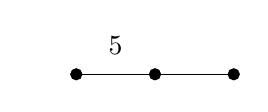
\begin{tikzpicture}[scale=1.0]
\draw[fill=black] \foreach \x in {1,2,...,3} {(\x,1.5) circle (2pt)};%H_{3}
\draw {(.5,1.5) node{}
(1.5,1.5) node[label=above:$5$]{}
[-] (1,1.5) -- (3,1.5)
(2,1.5) node{}}; 
\end{tikzpicture}
\caption{$H_{3}$} \label{fig:H}
\end{subfigure} &

\begin{subfigure}{0.5\textwidth} \centering
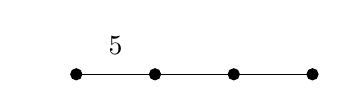
\begin{tikzpicture}[scale=1.0]
\draw[fill=black] \foreach \x in {1,2,...,4} {(\x,1.5) circle (2pt)};%H_{4}
\draw {(.5,1.5) node{}
(1.5,1.5) node[label=above:$5$]{}
[-] (1,1.5) -- (4,1.5)
(2,1.5) node{}}; 
\end{tikzpicture}
\caption{$H_{4}$} \label{fig:H}
\end{subfigure}
\end{tabular}
\caption{Irreducible finite Coxeter systems.}
\label{fig:fincoxgraphs}
\end{figure}

%%%%%%%%%%%%%%%%%%%%%%%%%%%

\begin{figure}[h!]
\begin{tabular}{m{7cm} m{7cm}}
\begin{subfigure}{0.5\textwidth} \centering
\begin{tikzpicture}[scale=1.0]%\widetilde{A}_{2}
\draw[fill=black] \foreach \x in {1,2} {(\x,10) circle (2pt)};
\fill[white] (1,11) circle (2pt);
\draw { (.5,10) node{}
(1.5,10) node[label=above:$\infty$]{}
%(1,10) node[label=below:$s_1$]{}
%(2,10) node[label=below:$s_2$]{}
[-] (1,10) -- (2,10)
(1,10) node{}}; 
\end{tikzpicture}
\caption{$\widetilde{A}_{2}$} \label{fig:affA2}
\end{subfigure} &

\begin{subfigure}{0.5\textwidth} \centering
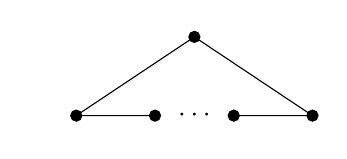
\begin{tikzpicture}[scale=1.0]%\widetilde{A}_{n}
\draw [fill=black] \foreach \x in {1,...,4} {(\x,7.5) circle (2pt)};
\draw [fill=black] (2.5, 8.5) circle (2pt);
\draw {(.5,8.5) node{}
(2.5,7.5) node{$\cdots$}
%(1,7.5) node[label=below:$s_1$]{}
%(2,7.5) node[label=below:$s_2$]{}
%(3,7.5) node[label=below:$s_{n-1}$]{}
%(4,7.5) node[label=below:$s_{n}$]{}
%(2.5,8.5) node[label=right:$s_{n+1}$]{}
[-] (2.5,8.5) -- (1, 7.5)
[-] (2.5,8.5) -- (4, 7.5)
[-] (1,7.5) -- (2,7.5)
[-] (3,7.5) -- (4,7.5)
(2,8.5) node{}}; 
\end{tikzpicture}
\caption{$\widetilde{A}_{n}$} \label{fig:affAn}
\end{subfigure} \\

    & \\ 

\begin{subfigure}{0.5\textwidth} \centering
\begin{tikzpicture}[scale=1.0]%\widetilde{B}_{n}
\draw[fill=black] \foreach \x in {1,2,...,6} {(\x,0) circle (2pt)};
\draw[fill=black] (5,1) circle (2pt);
\draw {(.25,0) node{}
(1.5,0) node[label=above:$4$]{}
(4.5, 0) node{$\cdots$}
%(1,0) node[label=below:$s_0$]{}
%(2,0) node[label=below:$s_1$]{}
%(3,0) node[label=below:$s_2$]{}
%(4,0) node[label=below:$s_3$]{}
%(5,0) node[label=below:$s_{n-2}$]{}
%(6,0) node[label=below:$s_{n-1}$]{}
%(5,1) node[label=right:$s_n$]{}
[-] (1,0) -- (4,0)
[-] (5,0) -- (6,0)
[-] (5,1) -- (5,0)
(2,0) node{}};
\end{tikzpicture}
\caption{$\widetilde{B}_{n}$} \label{fig:affB}
\end{subfigure} &

\begin{subfigure}{0.5\textwidth} \centering
\begin{tikzpicture}[scale=1.0]
\draw[fill=black] \foreach \x in {1,2,...,6} {(\x,5) circle (2pt)};%\widetild{C}_{n}
\fill[white] (1,6) circle (2pt);
\draw {(.5,5) node{}
(4.5,5) node{$\cdots$}
(5.5,5) node[label=above:$4$]{}
(1.5,5) node[label=above:$4$]{}
%(1,5) node[label=below:$s_0$]{}
%(2,5) node[label=below:$s_1$]{}
%(3,5) node[label=below:$s_2$]{}
%(4,5) node[label=below:$s_3$]{}
%(5,5) node[label=below:$s_{n-1}$]{}
%(6,5) node[label=below:$s_{n}$]{}
[-] (1,5) -- (4,5)
[-] (5,5) -- (6,5)
(2,5) node{}};
\end{tikzpicture}
\caption{$\widetilde{C}_{n}$} \label{fig:affC}
\end{subfigure} \\

    & \\ 
    
\begin{subfigure}{0.5\textwidth} \centering
\begin{tikzpicture}[scale=1.0]%\widetilde{D}_{6}
\draw[fill=black] \foreach \x in {1,2,...,6} {(\x,3.5) circle (2pt)};
\draw[fill=black] (2,4.5) circle (2pt);
\fill[white] (2,5.5) circle (2pt);
\draw[fill=black] (5,4.5) circle (2pt);
\draw {
(3.5,3.5) node{$\cdots$}
[-] (1,3.5) -- (3,3.5)
[-] (4, 3.5) --(6, 3.5)
[-] (2,3.5) -- (2,4.5)
[-] (5,3.5)-- (5,4.5)
(3,4.5) node{}};
\end{tikzpicture}
\caption{$\widetilde{D}_{n}$} \label{fig:E6}
\end{subfigure} &



\begin{subfigure}{0.5\textwidth} \centering
\begin{tikzpicture}[scale=1.0]%\widetilde{E}_{6}
\draw[fill=black] \foreach \x in {1,2,...,5} {(\x,4.5) circle (2pt)};
\draw[fill=black] (3, 5.5) circle (2pt);
\draw[fill=black] (3, 6.5) circle (2pt);
\draw {
[-] (1,4.5) -- (5,4.5)
[-] (3,4.5) -- (3,6.5)
(3,4.5) node{}};
\end{tikzpicture}
\caption{$\widetilde{E}_{6}$} \label{fig:affE6}
\end{subfigure} \\

    & \\ 


\begin{subfigure}{0.5\textwidth} \centering
\begin{tikzpicture}[scale=1.0]%\widetilde{E}_{7}
\draw[fill=black] \foreach \x in {1,2,...,7} {(\x,4.5) circle (2pt)};
\draw[fill=black] (4,5.5) circle (2pt);
\draw {
[-] (1,4.5) -- (7,4.5)
[-] (4,4.5) -- (4,5.5)
(3,4.5) node{}};
\end{tikzpicture}
\caption{$\widetilde{E}_{7}$} \label{fig:affE7}
\end{subfigure} &

\begin{subfigure}{0.5\textwidth} \centering
\begin{tikzpicture}[scale=1.0]%\widetilde{E}_{8}
\draw[fill=black] \foreach \x in {1,2,...,8} {(\x,3) circle (2pt)};
\draw[fill=black] (3,4) circle (2pt);
\draw {(.5,3) node{}
[-] (3,4) -- (3,3)
[-] (1,3) -- (8,3)
(3,3) node{}};
\end{tikzpicture}
\caption{$\widetilde{E}_{8}$} \label{fig:affE8}
\end{subfigure} \\

&\\

\begin{subfigure}{0.5\textwidth} \centering
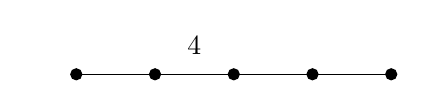
\begin{tikzpicture}[scale=1.0]
\draw[fill=black] \foreach \x in {1,2,...,5} {(\x,1.5) circle (2pt)};%\widetilde{F}_{4}
\draw {(.5,1.5) node{}
(2.5,1.5) node[label=above:$4$]{}
[-] (1,1.5) -- (5,1.5)
(2,1.5) node{}}; 
\end{tikzpicture}
\caption{$\widetilde{F}_{4}$} \label{fig:H}
\end{subfigure} &

\begin{subfigure}{0.5\textwidth} \centering
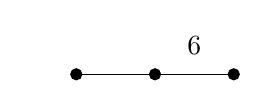
\begin{tikzpicture}[scale=1.0]
\draw[fill=black] \foreach \x in {1,2,...,3} {(\x,1.5) circle (2pt)};%\widetilde{G}_{2}
\draw {(.5,1.5) node{}
(2.5,1.5) node[label=above:$6$]{}
[-] (1,1.5) -- (3,1.5)
(2,1.5) node{}}; 
\end{tikzpicture}
\caption{$\widetilde{G}_{4}$} \label{fig:H}
\end{subfigure}
\end{tabular}
\caption{Irreducible affine Coxeter systems.}
\label{fig:infincoxgraphs}
\end{figure}


Given a Coxeter system $(W,S)$, a word $s_{x_1}s_{x_2} \cdots s_{x_m}$ in the free monoid $S^*$ on $S$ is called an \emph{expression} for $w \in W$ if it is equal to $w$ when considered as a group element. If $m$ is minimal among all expressions for $w$, the corresponding word is called a \emph{reduced expression} for $w$. In this case, we define the \emph{length} of $w$ to be $l(w):= m$. Each element $w \in W$ may have multiple reduced expressions that represent it. If we wish to emphasize a specific, possibly reduced, expression for $w \in W$ we will represent it as $\w=s_{x_1}s_{x_2}\cdots s_{x_m}$ (using {\sf{sans serif font}}). If $u,v \in W$, we say that the product $uv$ is \emph{reduced} if $l(uv)=l(u)+l(v)$. Matsumoto's Theorem, which follows, tells us more about how reduced expressions for a given group element are related.

\begin{proposition} [Matsumoto, \cite{Geck2000}]
	Let $(W,S)$ be a Coxeter system. If $w \in W$, then given a reduced expression for $w$ we can obtain every other reduced expression for $w$ by a sequence of braid moves and commutations of the form
	\[\underbrace{sts\cdots}_{m(s,t)} \rightarrow \underbrace{tst\cdots}_{m(s,t)}\]
	where $s,t \in S$ and $m(s,t) \geq 2$. \qed
\end{proposition}
 
It follows from Matsumoto's Theorem that if a generator $s$ appears in a reduced expression for $w \in W$, then $s$ appears in all reduced expressions for $w$. Let $w \in W$ and define the \emph{support} of $w$, denoted $\supp(w)$, to be the set of all generators that appear in any reduced expression for $w$. If $\supp(w)=S$, we say that $w$ has \emph{full support}. 

Given $w \in W$ and a fixed reduced expression $\w$ for $w$, any subsequence of $\w$ is called a \emph{subexpression} of $\w$. We will refer to a subexpression consisting of a consecutive subsequence of $\w$ as a \emph{subword} of $\w$. 

\begin{example}
Let $\w=s_7s_2s_4s_5s_3s_2s_3s_6$ be an expression for $w \in W(A_7)$. Then we have 
\begin{align*}
s_7\textcolor{purple}{s_2s_4}s_5s_3s_2s_3s_6&=s_7s_4\textcolor{purple}{s_2s_5}s_3s_2s_3s_6\\
&=s_7s_4s_5\textcolor{teal}{s_2s_3s_2} s_3s_6\\
&=s_7s_4s_5s_3s_2\textcolor{rred}{s_3s_3}s_6\\
&=s_7s_4s_5s_3s_2s_6,
\end{align*}
where the \textcolor{purple}{purple}-highlighted text corresponds to a commutation, the \textcolor{teal}{teal}-highlighted text corresponds to a braid move, and the \textcolor{rred}{red}-highlighted text corresponds to cancellation. This shows that the original expression $\w$ is not reduced. However, it turns out that $s_7s_4s_5s_3s_2s_6$ is reduced. Thus, $l(w)=6$ and $\supp(w)=\{s_2, s_3, s_4, s_5, s_6, s_7\}$.
\end{example}

Let $(W,S)$ be a Coxeter system and let $w \in W$. We define the \emph{left descent set} and \emph{right descent set} of $w$ as follows:
\[\mathcal{L}(w):=\{s \in S \mid l(sw) < l(w)\}\]

\[\mathcal{R}(w):=\{s \in S \mid l(ws) < l(w)\}.\]
In~\cite{Bjorner2005} it is shown that $s \in \mathcal{L}(w)$ (respectively, $\mathcal{R}(w)$) if and only if there is a reduced expression for $w$ that begins (respectively, ends) with $s$.

\begin{example}
The following list consists of all reduced expressions for a particular $w \in W(B_4)$:
$$\begin{array}{ll}
s_0s_1s_2s_1s_3 & s_0s_2s_1s_2s_3\\
s_0s_1s_2s_3s_1 & s_2s_0s_1s_2s_3	
\end{array}$$
We see that $l(w)=5$ and $w$ has full support. Also, we see that $\mathcal{L}(w)=\{s_0, s_2\}$ while $\mathcal{R}(w)=\{s_1, s_3\}$.	
\end{example}

Given a Coxeter system $(W,S)$, for any subset $I \subseteq S$, define $W_I$ to be the subgroup of $W$ generated by all $s \in I$. Such a subgroup is called a \emph{parabolic subgroup} of $W$. By Section 5.5 of~\cite{Humphreys1990}, for $I \subseteq S$, the corresponding parabolic subgroup forms a Coxeter system $(W_I,I)$ with the given values $m(s,t)$.
%%%%%%%%%%%%%%%%%%%%%%%%%%%


\section{Fully Commutative Elements}\label{sec:FC}
Let $(W,S)$ be a Coxeter system of type $\Gamma$ and let $w \in W(\Gamma)$. Following~\cite{Stembridge1996}, we define a relation $\sim$ on the set of reduced expressions for $w$. Let $\w_1$ and $\w_2$ be two reduced expressions for $w$. We define $\w_1 \sim \w_2$ if we can obtain $\w_2$ from $\w_1$ by applying a single commutation move of the form $st \mapsto ts$ where $m(s,t)=2$. Now, define the equivalence relation $\approx$ by taking the reflexive transitive closure of $\sim$. Each equivalence class under $\approx$ is called a \emph{commutation class}. If there is a single commutation class for the set of reduced expressions for $w$, then we say that $w$ is \emph{fully commutative} (FC). 

The set of FC elements of $W(\Gamma)$ is denoted by $\FC(\Gamma)$. Given some $w \in \FC(\Gamma)$ and a starting reduced expression for $w$, observe that the definition of FC states that one only needs to perform commutations to obtain all reduced expressions for $w$, but the following result due to Stembridge~\cite{Stembridge1996} states that when $w$ is FC, performing commutations is the only possible way to obtain another reduced expression for $w$.

\begin{proposition}[Stembridge,~\cite{Stembridge1996}]\label{thm:Stembridge}
	An element $w \in \FC(\Gamma)$ is FC if and only if no reduced expression for $w$ contains $\underbrace{sts\cdots}_{m(s,t)}$ as a subword for all $m(s,t) \geq 3$. \qed
\end{proposition}

In other words, $w$ is FC if and only if no reduced expression provides the opportunity to apply a braid move. For example, in a Coxeter system of type $B_n$ an element is $\FC$ if no reduced expression contains the subwords $s_0s_1s_0s_1$, $s_1s_0s_1s_0$, $s_ks_{k+1}s_k$, and $s_{k+1}s_ks_{k+1}$ where $0<k\leq n-2$. In a Coxeter system of type $\C_n$, an element is $\FC$ if no reduced expression for the element contains the subwords seen above with $0<k\leq n-1$ and does not contain the subwords $s_{n-1}s_ns_{n-1}s_n$ and $s_{n}s_{n-1}s_ns_{n-1}$.

%\begin{example}
%	\textcolor{green}{Let $\w=s_0s_1s_2s_0s_3s_1$ be a reduced expression for $w \in W(\C_4)$}. Although it is not immediately obvious, there is no possible way to perform a braid move in any reduced expression for $w$. Hence $w$ is $\FC$.
%\end{example}

\begin{example}
Let $\w_1=s_1s_0s_1s_3s_4s_5s_2s_4s_6$ be a reduced expression for $w \in W(\widetilde{C}_6)$. Applying the commutation $s_2s_4 \mapsto s_4s_2$, we can obtain another reduced expression for $w$, namely $\w_2=s_1s_0s_1s_3s_4s_5s_4s_2s_6$, which is in the same commutation class as $\w_1$. However, applying the braid move $s_4s_5s_4 \mapsto s_5s_4s_5$, we obtain another reduced expression $\w_3=s_1s_0s_1s_3s_5s_4s_5s_2s_6$. Note that since $\w_3$ was obtained by applying a braid move, $\w_3$ is in a different commutation class from $\w_1$ and $\w_2$. Since $w$ has at least two commutation classes, one containing $\w_1$ and $\w_2$ and another containing $\w_3$, $w$ is not FC by Proposition~\ref{thm:Stembridge}.
\end{example}

%\begin{example}
%Let $w \in W(\widetilde{C}_4)$ and let $\w=s_0s_1s_2s_0s_1s_2$ be a reduced expression for $w$. We see that
%\[s_0s_1\textcolor{purple}{s_3s_0}s_1s_2=s_0s_1s_0\textcolor{purple}{s_3s_1}s_2=\textcolor{orange}{s_0s_1s_0s_1}s_3s_2,\]
%where the \textcolor{purple}{purple}-highlighted text indicates applying a commutation and the \textcolor{orange}{orange}-highlighted text indicates applying a braid move. Thus, $w$ is not $\FC$ by Theorem~\ref{thm:Stembridge}.  	
%\end{example}

Stembridge classified the Coxeter systems whose groups contain a finite number of FC elements, the so-called \emph{FC-finite Coxeter groups}. Both $W(A_n)~\mathrm{and}~W(B_n)$ are finite Coxeter groups, and Thus, are $\FC$-finite. On the other hand, $W(\widetilde{C}_n)$ is infinite and happens to also contain infinitely many $\FC$ elements. There exist infinite Coxeter groups that contain finitely many $\FC$ elements. For example, $W(E_n$) for $n \geq 9$ (see Figure~\ref{fig:FCfincoxgraphs}) is infinite, but contains only finitely many FC elements.

\begin{proposition}[Stembridge,~\cite{Stembridge1996}]
\label{thm:FCfinite} The irreducible FC-finite Coxeter systems are of type $A_n$ with $n \geq 1$, $B_n$ with $n \geq 2$, $D_n$ with $n \geq 4$, $E_n$ with $n \geq 6$, $F_n$ with $n \geq 4$, $H_n$ with $n \geq 3$, and $I_2(m)$ with $5 \leq m < \infty$. \qed
\end{proposition} 
 
The irreducible FC-finite Coxeter graphs are given in Figure~\ref{fig:FCfincoxgraphs}. Note that the irreducible finite Coxeter systems given in Figure~\ref{fig:fincoxgraphs} certainly have only a finite number of FC elements. So the irreducible FC-finite Coxeter systems contain the irreducible finite Coxeter systems. However, notice there are a few graphs in Figure~\ref{fig:fincoxgraphs} that we have not yet encountered. Specifically, we have not yet encountered the Coxeter groups determined by graphs in Figures~\ref{fig:FCEn} for $n \geq 9$,~\ref{fig:FCFn} for $n \geq 5$,~\ref{fig:FCHn} for $n \geq 5$. All of these Coxeter systems have corresponding infinite groups for sufficiently large $n$, yet contain only finitely many FC elements.

\begin{figure}[h!]
\begin{tabular}{m{7cm} m{7cm}}
\begin{subfigure}{0.5\textwidth} \centering
\begin{tikzpicture}[scale=1.0]%A_{n}
\draw[fill=black] \foreach \x in {1,2,...,6} {(\x,10) circle (2pt)};
\draw {(.5,10) node{}
(1.5,10) node[label=above:\textcolor{white}{$4$}]{}
(4.5,10) node{$\cdots$}
[-] (1,10) -- (4,10)
[-] (5,10) -- (6,10)
(1,10) node{}}; 
\end{tikzpicture}
\caption{$A_{n}$} \label{fig:FCA}
\end{subfigure} &

\begin{subfigure}{0.5\textwidth} \centering
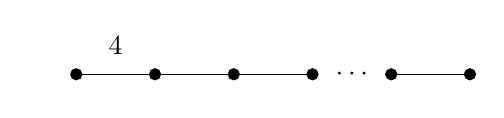
\begin{tikzpicture}[scale=1.0]%B_{n}
\draw [fill=black] \foreach \x in {1,2,...,6} {(\x,8.5) circle (2pt)};
\draw {(.5,8.5) node{}
(1.5,8.5) node[label=above:$4$]{}
(4.5,8.5) node{$\cdots$}
[-] (1,8.5) -- (4,8.5)
[-] (5,8.5) -- (6,8.5)
(2,8.5) node{}}; 
\end{tikzpicture}
\caption{$B_{n}$} \label{fig:FCB}
\end{subfigure} \\

    & \\ 

\begin{subfigure}{0.5\textwidth} \centering
\begin{tikzpicture}[scale=1.0]
\draw[fill=black] \foreach \x in {1,2,...,6} {(\x,6.5) circle (2pt)};%D_{n}
\draw[fill=black] (2,7.5) circle (2pt);
\draw {(.5,6.5) node{}
(4.5,6.5) node{$\cdots$}
[-] (1,6.5) -- (4,6.5)
[-] (5,6.5) -- (6,6.5)
[-] (2,6.5) -- (2,7.5)
(2,6.5) node{}};
\end{tikzpicture}
\caption{$D_{n}$} \label{fig:FCD}
\end{subfigure} &
    
\begin{subfigure}{0.5\textwidth} \centering
\begin{tikzpicture}[scale=1.0]%E_{6}
\draw[fill=black] \foreach \x in {1,2,...,6} {(\x,4.5) circle (2pt)};
\draw[fill=black] (3,5.5) circle (2pt);
%\fill[white] (3,5.9) circle (2pt);
\draw {(.5, 4.5) node{}
(4.5,4.5) node{$\cdots$}
[-] (1,4.5) -- (4,4.5)
[-] (5,4.5) -- (6,4.5)
[-] (3,4.5) -- (3,5.5)
(3,4.5) node{}};
\end{tikzpicture}
\caption{$E_{n}$} \label{fig:FCEn}
\end{subfigure} \\

&\\

\begin{subfigure}{0.5\textwidth} \centering
\begin{tikzpicture}[scale=1.0]%F_{n}
\draw[fill=black] \foreach \x in {1,2,...,6} {(\x,3) circle (2pt)};
\fill[white] (1,4) circle (2pt);
\draw {(.5,3) node{}
(2.5,3) node[label=above:$4$]{}
(4.5,3) node{$\cdots$}
[-] (1,3) -- (4,3)
[-] (5,3) -- (6,3)
(3,3) node{}};
\end{tikzpicture}
\caption{$F_{n}$} \label{fig:FCFn}
\end{subfigure} &


\begin{subfigure}{0.5\textwidth} \centering
\begin{tikzpicture}[scale=1.0]
\draw[fill=black] \foreach \x in {1,2,...,6} {(\x,1.5) circle (2pt)};%H_{4}
\fill[white] (1,2.5) circle (2pt);
\draw {(.5,1.5) node{}
(1.5,1.5) node[label=above:$5$]{}
(4.5,1.5) node{$\cdots$}
[-] (1,1.5) -- (4,1.5)
[-] (5,1.5) -- (6,1.5)
(2,1.5) node{}}; 
\end{tikzpicture}
\caption{$H_{n}$} \label{fig:FCHn}
\end{subfigure}\\

&\\
\end{tabular}

\begin{subfigure}{1.0\textwidth} \centering
\begin{tikzpicture}[scale=1.0]
\draw[fill=black] \foreach \x in {1,2} {(\x,0) circle (2pt)};
\fill[fill=white] (2,1) circle (2pt);
\draw {(.25,0) node{}
(1.5,0) node[label=above:$m$]{}
[-] (1,0) -- (2,0)
(2,0) node{}};
\end{tikzpicture}
\caption{$I_{2}(m)$} \label{fig:FCI}
\end{subfigure}

\caption{Irreducible FC-finite Coxeter systems.}
\label{fig:FCfincoxgraphs}
\end{figure}


%%%%%%%%%%%%%%%%%%%%%%%%%%%%%%%%
\section{Heaps}\label{sec:Heaps}

We now discuss a visual representation of Coxeter group elements. Each reduced expression can be associated with a labeled partially ordered set (poset) called a heap.  Heaps provide a visual representation of a reduced expression while preserving the relations among the generators. We follow the development of heaps for straight-line Coxeter groups found in~\cite{Billey2007},~\cite{Ernst2010}, and~\cite{Stembridge1996}. 

Let $(W,S)$ be a Coxeter system of type $\Gamma$. Suppose $\w=s_{x_1}s_{x_2}\cdots s_{x_r}$ is a fixed reduced expression for $w \in W(\Gamma)$. As in~\cite{Stembridge1996}, we define a partial ordering on the indices $\{1, 2, \ldots, r\}$ by the transitive closure of the relation $\lessdot$ defined via $j \lessdot i$ if $i < j$ and $s_{x_i}$ and $s_{x_j}$ do not commute. In particular, since $\w$ is reduced, $j \lessdot i$ if $s_{x_i}=s_{x_j}$ by transitivity. This partial order is referred to as the \emph{heap} of $\w$, where $i$ is labeled by $s_{x_i}$. Note that for simplicity we are omitting the labels of the underlying poset yet retaining the labels of the corresponding generators.

It follows from~\cite{Stembridge1996} that heaps are well-defined up to commutation class. That is, given two reduced expressions $\w_1$ and $\w_2$ for $w \in W$ that are in the same commutation class, the heaps for $\w_1$ and $\w_2$ will be equal. In particular, if $w \in \FC(\Gamma)$, then $w$ has one commutation class, and Thus, $w$ has a unique heap. Conversely, if $\w_1$ and $\w_2$ are in different commutation classes, then the heap of $\w_1$ will be distinct from the heap of $\w_2$.

\begin{example}\label{ex:word}
Let $\w=s_6s_4s_2s_5s_3s_1s_4s_0s_1$ be a reduced expression for $w \in \FC(\widetilde{C}_6).$ We see that $\w$ is indexed by $\{1,2,3,4,5,6,7,8,9\}$. As an example, $9 \lessdot 8$ since $8 <9$ and $s_0$ and $s_1$ do not commute. The labeled Hasse diagram for the heap poset is seen in Figure~\ref{fig:Hasse}.
\begin{figure}[h]
\centering
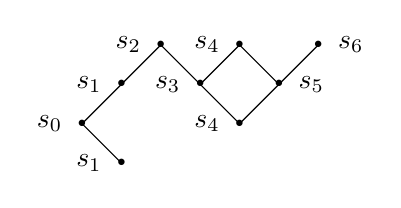
\begin{tikzpicture}[scale=0.5]
	\node[scale=0.6, label=left:$s_{2}$] at (2,5.5) {$\bullet$};
	\node[scale=0.6, label=left:$s_{4}$] at (4,5.5) {$\bullet$};
	\node[scale=0.6, label=right:$s_{6}$] at (6,5.5) {$\bullet$};
	\node[scale=0.6, label=left:$s_{1}$] at (1,4.5) {$\bullet$};
	\node[scale=0.6, label=left:$s_{3}$] at (3,4.5) {$\bullet$};
	\node[scale=0.6, label=right:$s_{5}$] at (5,4.5) {$\bullet$};
	\node[scale=0.6, label=left:$s_{0}$] at (0,3.5) {$\bullet$};
	\node[scale=0.6, label=left:$s_{4}$] at(4,3.5) {$\bullet$};
	\node[scale=0.6, label=left:$s_{1}$] at (1,2.5) {$\bullet$};
\draw (1,2.5)--(0,3.5)--(1,4.5)--(2,5.5)--(3,4.5)--(4,3.5);
\draw (3,4.5)--(4,5.5)--(5,4.5)--(4,3.5);
\draw (6,5.5)--(5,4.5);
\end{tikzpicture}
\caption{Labeled Hasse diagram for the heap of an element in $\FC(\widetilde{C}_6).$}
\label{fig:Hasse}	
\end{figure}
\end{example}

Let $\w$ be a reduced expression for an element $w \in W(\widetilde{C}_n)$. As in~\cite{Billey2007} and~\cite{Ernst2010} we can represent a heap of $\w$ as a set of lattice points embedded in $\{0,1,2,\ldots, n\} \times \mathbb{N}$. To do so, we assign coordinates (not unique) $(x,y) \in \{0,1,2,\ldots, n\} \times \mathbb{N}$ to each entry of the labeled Hasse diagram for the heap of $\w$ in such a way that:
\begin{enumerate}[leftmargin=2cm]
\item An entry with coordinates $(x,y)$ is labeled $s_i$ (or $i$) in the heap if and only if $x = i$; 

\item If an entry with coordinates $(x,y)$ is greater than an entry with coordinates $(x',y')$ in the heap then $y > y'$.
\end{enumerate}

Although the above is specific to $W(\widetilde{C}_n)$, the same construction works for any straight-line Coxeter graph with the appropriate adjustments made to the label set and assignment of coordinates. Specifically, for type $A_n$ our label set is $\{1,2, \ldots, n\}$ and for type $B_n$ our label set is $\{0,1, \ldots, n-1\}$.

In the case of any straight-line Coxeter graph, it follows from the definition that $(x,y)$ covers $(x',y')$ in the heap if and only if $x = x' \pm 1$, $y'< y$, and there are no entries $(x'', y'')$ such that $x'' \in \{x, x'\}$ and $y'< y'' < y$. This implies that we can completely reconstruct the edges of the Hasse diagram and the corresponding heap poset from a lattice point representation. The lattice point representation can help us visualize arguments that are potentially complex. Note that in our heaps the entries fully exposed to the top (respectively, bottom) correspond to the generators occurring in the left (respectively, right) descent set of the corresponding reduced expression.

Let $\w$ be a reduced expression for $w \in W(\widetilde{C}_n)$. We denote the lattice point representation of the heap poset in $\{0,1,2, \ldots n\} \times \mathbb{N}$ described in the preceding paragraphs via $H(\w)$. If $w$ is $\FC$, then the choice of reduced expression for $w$ is irrelevant and we will often write $H(w)$ and we refer to $H(w)$ as the heap of $w$. Note that we will use the same notation for heaps in Coxeter groups of all types with straight-line Coxeter graphs.

Let $\w=s_{x_1}s_{x_2}\cdots s_{x_r}$ be a reduced expression for $w \in W(\widetilde{C}_n)$. If $s_{x_i}$ and $s_{x_j}$ are adjacent generators in the Coxeter graph with $i<j$, then we must place the point labeled by $s_{x_i}$ at a level that is \emph{above} the level of the point labeled by $s_{x_j}$. Because generators in a Coxeter graph that are not adjacent do commute, points whose $x$-coordinates differ by more than one can slide past each other or land in the same level. To emphasize the covering relations of the lattice point representation we will enclose each entry in the heap in a square with rounded corners (called a block) in such a way that if one entry covers another the blocks overlap halfway. In addition, we will also label each square for $s_i$ with $i$.

There are potentially many ways to illustrate a heap of an arbitrary reduced expression, each differing by the vertical placement of the blocks. For example, we can place blocks in vertical positions as high as possible, as low as possible, or some combination of low/high. In this thesis, we choose what we view to be the best representation of the heap of each example and when illustrating the heaps of arbitrary reduced expressions we will discuss the relative position of the entries but never the absolute coordinates.

We say that a block in the heap for a reduced expression is \emph{fully exposed} to the top (respectively, bottom) to mean that the top (respectively, bottom) edge of a heap block is not covered by any blocks above (respectively, below) in the heap. That is, there are no blocks that cover part of the top or bottom edge of the heap. Since there are multiple heap representations when $w \in W(\Gamma)$ is not FC, it is possible that a block that is fully exposed in one heap may not be fully exposed in a different heap representing $w$. 

\begin{example}
	Let $\w=s_6s_4s_2s_5s_3s_1s_4s_0s_1$ be a reduced expression for $w \in \FC(\widetilde{C}_6)$ as seen in Example~\ref{ex:word}. Figure~\ref{fig:FC heap} shows a possible lattice point representation for $H(\w)$. Since $w$ is FC this is the unique heap representation for $w$. Because $\w$ has a unique heap, we can obtain $\LD(w)$ (respectively, $\RD(w)$) from the blocks that are fully exposed to the top (respectively, bottom) of the heap. We see that $\LD(w)=\{s_2,s_4,s_6\}$ and $\RD(w)=\{s_1,s_4\}$.
\begin{figure}[h]
\centering
\begin{tikzpicture}[scale=0.45]
\heapblock{2}{6}{2}{purple}
\heapblock{4}{6}{4}{purple}
\heapblock{6}{6}{6}{purple}
\heapblock{1}{4}{1}{purple}
\heapblock{3}{4}{3}{purple}
\heapblock{5}{4}{5}{purple}
\heapblock{0}{2}{0}{purple}
\heapblock{4}{2}{4}{purple}
\heapblock{1}{0}{1}{purple}
\end{tikzpicture}
\caption{A lattice point representation for the heap of an FC element in $W(\widetilde{C}_6)$.}
\label{fig:FC heap}
\end{figure}
\end{example}

\begin{example}
Let $\w_1=s_0s_2s_4s_3s_2s_1$ be a reduced expression for $w \in W(\widetilde{C}_4)$. Applying the commutation move $s_2s_4\mapsto s_4s_2$, we can obtain another reduced expression for $w$, namely $\w_2=s_0s_4s_2s_3s_2s_1$, which is in the same commutation class as $\w_1$, and hence has the same heap. However, applying the braid move $s_2s_3s_2 \mapsto s_3s_2s_3$, we obtain another reduced expression $\w_3=s_0s_4s_3s_2s_3s_1$. Note that since $\w_3$ was obtained by applying a braid move, $\w_3$ is in a different commutation class than $\w_1$ and $\w_2$. Representations of $H(\w_1), H(\w_2)$, and $H(\w_3)$ are seen in Figure~\ref{fig:not FC}, where the braid relation is colored in \textcolor{teal}{teal}. From the heaps we see that $\LD(w)=\{s_0,s_2,s_4\}$ and $\RD=\{s_1,s_3\}$. However, if we only had one heap or the other, we would miss some elements in the left and right descent sets as $s_3$ is not fully exposed to the bottom of the heap in Figure~\ref{fig:notFC2} and $s_2$ is not fully exposed to the top of the heap in Figure~\ref{fig:notFC3}. 

\begin{figure}[h]
\centering
\begin{subfigure}[b]{0.3\textwidth}	
\centering
\begin{tikzpicture}[scale=0.45]
\heapblock{0}{6}{0}{purple}
\heapblock{2}{6}{2}{teal}
\heapblock{4}{6}{4}{purple}	
\heapblock{3}{4}{3}{teal}
\heapblock{2}{2}{2}{teal}
\heapblock{1}{0}{1}{purple}
\end{tikzpicture}
\caption{$H(\w_1)$ and $H(\w_2)$.}\label{fig:notFC2}
\end{subfigure}
\begin{subfigure}[b]{0.3\textwidth}	
\centering
\begin{tikzpicture}[scale=0.45]
\heapblock{10}{6}{0}{purple}
\heapblock{14}{6}{4}{purple}
\heapblock{13}{4}{3}{teal}
\heapblock{12}{2}{2}{teal}
\heapblock{11}{0}{1}{purple}
\heapblock{13}{0}{3}{teal}
\end{tikzpicture}
\caption{$H(\w_3)$}\label{fig:notFC3}
\end{subfigure}
\caption{Two heaps of a non-FC element in $W(\widetilde{C}_4)$.}	
\label{fig:not FC}
\end{figure}
\end{example}

As for expressions, it will be helpful to have the notion of a subheap. Let $\w=s_{x_1}s_{x_2} \cdots s_{x_r}$ be a reduced expression for $w \in W(\Gamma)$. We define a heap $H'$ to be a \emph{subheap} of $H(\w)$ if $H'=H(\w')$ where $\w'=s_{y_1}s_{y_2} \cdots s_{y_k}$ is a subexpression of $\w$. We emphasize that the subexpression need not be a subword (i.e., a consecutive subexpression).

Recall that a subposet $Q$ of $P$ is called convex if $y \in Q$ whenever $x< y<z$ in $P$ and $x,z \in Q$. We will refer to a subheap as a \emph{convex subheap} if the underlying subposet is convex.

\begin{example}
Let $\w=s_3s_2s_1s_2s_5s_4s_6s_5$ be a reduced expression for $w \in W(\C_7)$. Now let $\w'=s_5s_4s_5$ be the subexpression of $\w$ that results from deleting all but the fifth, sixth, and last generators of $\w$. Then the subheap $H(\w')$ is seen in Figure~\ref{fig:subheap}. However, $H(\w')$ is not convex since there is an entry in $H(w)$ labeled by $s_6$ occurring between the two consecutive occurrences of $s_5$ that does not occur in $H(w')$. However, if we do include the entry labeled by $s_6$, then we get the subheap seen in Figure~\ref{fig:convex}, which is convex.

\begin{figure}[h]
\centering
\begin{subfigure}[b]{0.3\textwidth}	
\centering
\begin{tikzpicture}[scale=0.45]
%	\heapblock{0}{6}{0}{purple}
%	\heapblock{2}{6}{2}{teal}
%	\heapblock{4}{6}{4}{purple}	
	\heapblock{3}{4}{5}{purple}
	\heapblock{2}{2}{4}{purple}
	\heapblock{3}{0}{5}{purple}
\end{tikzpicture}
\caption{}\label{fig:subheap}
\end{subfigure}
\begin{subfigure}[b]{0.3\textwidth}	
\centering
\begin{tikzpicture}[scale=0.45]
%	\heapblock{10}{6}{0}{purple}
%	\heapblock{14}{6}{4}{purple}
	\heapblock{13}{4}{5}{purple}
	\heapblock{12}{2}{4}{purple}
	\heapblock{14}{2}{6}{purple}
	\heapblock{13}{0}{5}{purple}
\end{tikzpicture}
\caption{}\label{fig:convex}
\end{subfigure}
\caption{Subheap and convex subheap of the heap for an element in $W(\C_7)$.}	
\end{figure}
\end{example}


It will be extremely useful for us to be able to quickly determine whether a heap corresponds to an element in $\FC(B_n)$ or $\FC(\widetilde{C}_n)$. The next proposition is a special case of \cite[Proposition 3.3]{Stembridge1996} and follows easily when one considers the consecutive subwords that are impermissible in reduced expressions for elements in $\FC(B_n)$ and $\FC(\widetilde{C}_n)$ as discussed in Section~\ref{sec:FC}.

\begin{proposition}
Let $(W,S)$ be a Coxeter system of type $\C_n$. If $w \in \FC(\widetilde{C}_n)$, then $H(w)$ cannot contain any of the configurations seen in Figure~\ref{fig:impermiss heaps}, where $0 < k < n-1$ and we use a square with a dotted boundary to emphasize that no element of the heap may occupy the corresponding position. \qed
\end{proposition}

\begin{figure}[h]
\begin{tabular}{m{4cm} m{4cm} m{4cm}}
	\begin{subfigure}{0.33\textwidth} \centering
	\begin{tikzpicture}[scale=0.45]
		\heapblock{1}{6}{1}{purple}
		\dheapblock{2}{4}{}{black}
		\heapblock{0}{4}{0}{purple}
		\heapblock{1}{2}{1}{purple}
		\heapblock{0}{0}{0}{purple}
	\end{tikzpicture}
	\caption{}\label{fig:C&B}
	\end{subfigure} &
	
	\begin{subfigure}{0.33\textwidth} \centering
	\begin{tikzpicture}[scale=0.45]
		\heapblock{0}{6}{0}{purple}
		\heapblock{1}{4}{1}{purple}
		\heapblock{0}{2}{0}{purple}
		\dheapblock{2}{2}{}{black}
		\heapblock{1}{0}{1}{purple}
	\end{tikzpicture}
	\caption{}\label{fig:C&B2}
	\end{subfigure} &

	\begin{subfigure} {0.33\textwidth} \centering
	\begin{tikzpicture}[scale=0.45]
		\heapblock{1}{8}{}{white}
		\heapblock{1}{6}{k+1}{purple}
		\heapblock{0}{4}{k}{purple}
		\dheapblock{2}{4}{}{black}
		\heapblock{1}{2}{k+1}{purple}
	\end{tikzpicture}
	\caption{}\label{fig:a,b,c}
	\end{subfigure}\\
	
	&\\
	
	\begin{subfigure}{0.33\textwidth} \centering
	\begin{tikzpicture}[scale=0.45]
		\heapblock{1}{8}{}{white}
		\heapblock{2}{6}{k}{purple}
		\heapblock{3}{4}{k+1}{purple}
		\dheapblock{1}{4}{}{black}
		\heapblock{2}{2}{k}{purple}
	\end{tikzpicture}
	\caption{}\label{fig:a,b,c2}
	\end{subfigure}&
	
	\begin{subfigure}{0.33\textwidth} \centering
	\begin{tikzpicture}[scale=0.45]
		\heapblock{2}{6}{n}{purple}
		\heapblock{1}{4}{n-1}{purple}
		\heapblock{2}{2}{n}{purple}
		\dheapblock{0}{2}{}{black}
		\heapblock{1}{0}{n-1}{purple}
	\end{tikzpicture}
	\caption{}\label{fig:cimpermiss}	
	\end{subfigure} &
	
	\begin{subfigure}{0.33\textwidth} \centering
	\begin{tikzpicture}[scale=0.45]
		\heapblock{1}{6}{n-1}{purple}
		\dheapblock{0}{4}{}{black}
		\heapblock{2}{4}{n}{purple}
		\heapblock{1}{2}{n-1}{purple}
		\heapblock{2}{0}{n}{purple}
	\end{tikzpicture}	
	\caption{}\label{fig:cimpermiss2}
	\end{subfigure}
\end{tabular}	
\caption{Impermissible configurations for heaps of $\FC(\widetilde{C}_n)$.}\label{fig:impermiss heaps}
\end{figure}

Since $W(B_n)$ is a parabolic subgroup of $W(\widetilde{C}_n)$, we can use Figure~\ref{fig:impermiss heaps} to classify the impermissible configurations for elements of $\FC(B_n)$. In particular, the impermissible configurations for elements of $\FC(B_n)$ are those seen in Figures~\ref{fig:C&B},~\ref{fig:C&B2}~\ref{fig:a,b,c}, and~\ref{fig:a,b,c2}. 

